\subsection{Topology Skeletons}
\begin{frame}[fragile]{Simple Pipe}
A simple Pipe (without Futures):
\begin{lstlisting}[frame=htrbl]
pipeSimple :: conf -> [arr a a] -> arr a a
pipeSimple conf fs =
  loop (arr snd &&&
    (arr (uncurry (:) >>> lazy) >>> loopParEvalN conf fs)) >>>
  arr last
\end{lstlisting}
\end{frame}
\begin{frame}[fragile]{Pipe with Futures}
With Futures we get inter-node communication:
\begin{lstlisting}[frame=htrbl]
pipe :: conf -> [arr a a] -> arr a a
pipe conf fs =
	unliftFut conf (pipeSimple conf (map (liftFut conf) fs))
\end{lstlisting}
We can even implement
\begin{lstlisting}[frame=htrbl]
pipe2 :: conf -> arr a b -> arr b c -> arr a c|
\end{lstlisting}
Which gives us parallel composition:
\begin{lstlisting}[frame=htrbl]
(|>>>|) :: arr a b -> arr b c -> arr a c
(|>>>|) = pipe2 ()
\end{lstlisting}
\end{frame}
\begin{frame}[fragile]{Ring}
\begin{center}
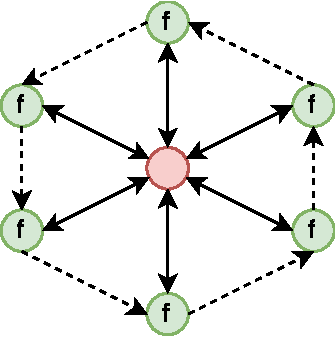
\includegraphics[scale=0.8]{images/ring.pdf}
\end{center}
\end{frame}
\begin{frame}[fragile]{Torus}
\begin{center}
\includegraphics[scale=0.8]{images/torus.pdf}
\end{center}
\end{frame}